\documentclass[a4paper,10pt]{article}
\usepackage[utf8x]{inputenc}
\usepackage{amssymb}
\usepackage{xlop}
\usepackage{xcolor}
\input{longdiv}
\usepackage{graphicx}
\usepackage{wrapfig}
\usepackage{float}

%opening
\title{Examen de evaluación}
\author{}
\date{}
\begin{document}
\maketitle
\subsection*{Aritmética}

 \subsubsection*{Enteros}

\opadd[resultstyle=\color{white},carrystyle=\color{white}]{9}{7} \hspace{1.5cm}
\opadd[resultstyle=\color{white},carrystyle=\color{white}]{79}{48}\hspace{1.5cm}
\opadd[resultstyle=\color{white},carrystyle=\color{white}]{268}{79}\hspace{1.5cm}
\vspace{1.5cm} \\
\opsub[resultstyle=\color{white},carrystyle=\color{white}]{7}{3}\hspace{1.5cm} 
\opsub[resultstyle=\color{white},carrystyle=\color{white}]{49}{8}\hspace{1.5 cm}
\opsub[resultstyle=\color{white},carrystyle=\color{white}]{168}{97}\hspace{1.5cm}
\vspace{1.5cm} \\
\opmul[resultstyle=\color{white},carrystyle=\color{white}]{7}{8}\hspace{1.5cm} 
\opmul[resultstyle=\color{white},carrystyle=\color{white}]{73}{8}\hspace{1.5cm}
\opmul[resultstyle=\color{white},carrystyle=\color{white}, displayintermediary=None]{143}{68}\hspace{1.5cm}
\vspace{1.5cm} \\
$3\;\vline \overline{\;27}$\hspace{1.5cm}
$7\;\vline \overline{\;8 4}$\hspace{1.5cm}
$12\;\vline \overline{\;5 4 6}$\hspace{1.5cm}
\\ 
\subsubsection*{Decimales}
\opadd[resultstyle=\color{white},carrystyle=\color{white}]{0.3}{0.7}\hspace{1.5cm} 
\opadd[resultstyle=\color{white},carrystyle=\color{white}]{4.9}{0.3}\hspace{1.5cm} 
\opadd[resultstyle=\color{white},carrystyle=\color{white}]{2.38}{7.03}\hspace{1.5cm}
\vspace{1.5cm} \\
\opsub[resultstyle=\color{white},carrystyle=\color{white}]{0.7}{0.4}\hspace{1.5cm} 
\opsub[resultstyle=\color{white},carrystyle=\color{white}]{2.2}{0.8}\hspace{1.5cm} 
\opsub[resultstyle=\color{white},carrystyle=\color{white}]{3.2}{0.4}\hspace{1.5cm}
 \vspace{1.5cm} \\
\opmul[resultstyle=\color{white},carrystyle=\color{white},displayintermediary=None]{3}{0.7}\hspace{1.5cm}
\opmul[resultstyle=\color{white},carrystyle=\color{white},displayintermediary=None]{2.3}{0.7}\hspace{1.5cm} 
\opmul[resultstyle=\color{white},carrystyle=\color{white},displayintermediary=None]{2.53}{7.9}\hspace{1.5cm}
 \vspace{1.5cm} \\
$3\;\vline \overline{\;2.7}$\hspace{1.5cm}
$0.7\;\vline \overline{\;8 4}$\hspace{1.5cm}
$1.2\;\vline \overline{\;5.46}$\hspace{1.5cm}
\\
\subsubsection*{Fracciones}
decimal a fraccion  $0.5=$\hspace{1.5cm}
fraccion a decimal  $\frac{7}{4}=$\hspace{1.5cm}
 \vspace{1cm}\\
a fraccion impropia $1\frac{2}{3}=$\hspace{1.5cm}
a fraccion propia   $\frac{7}{6}=$\hspace{1.5cm}
\vspace{1cm}\\
$\frac{2}{8}+\frac{4}{8}=$\hspace{3cm}
$\frac{2}{5}+\frac{4}{15}=$\hspace{3cm}
$1\frac{7}{12}+\frac{2}{24}=$\hspace{3cm}
\vspace{1cm}\\
$\frac{7}{9}-\frac{2}{9}=$\hspace{3cm}
$\frac{2}{7}-\frac{4}{14}=$\hspace{3cm}
$1\frac{3}{15}+\frac{17}{30}=$\hspace{3cm}
\vspace{1cm}\\
$\frac{2}{5}\cdot\frac{3}{5}=$\hspace{2cm}
$1\frac{2}{7}\cdot\frac{3}{4}=$\hspace{2cm}
$\frac{3}{15} \div\frac{2}{13}=$\hspace{2cm}
$1\frac{3}{7} \div\frac{5}{40}=$\hspace{2cm}

\subsubsection*{Negativos}
$5+(-3)=$\hspace{2cm}$-5+4=$ \hspace{2cm} $-1\times -3=$\hspace{2cm} $4\times -7=$

\subsubsection*{Potencias}
$3^2=$\hspace{2cm}
$2^5=$

\subsubsection*{Raíces}
$\sqrt{9}=$\hspace{2cm}
$\sqrt[3]{8}=$\hspace{2cm}

\subsubsection*{Logaritmos}
$\log_2{8}=$\hspace{2cm}
$\log_{10}100=$

\subsection*{Álgebra}

\subsubsection*{Operaciones básicas}
$a+a=$\hspace{2cm} $a+ab+a+b=$ \hspace{2cm} $2z+3x+4z=$
\vspace{1cm}\\
$a\times b=$\hspace{2cm} $ab\times ab=$ \hspace{2cm} $xy\times x = $
\vspace{1cm}\\
$\frac{ab}{b}$ \hspace{2cm} $\frac{a^2}{ab}=$ \hspace{2cm} $\frac{x^2}{x}=$ \hspace$\frac{a^2-ba}{a}$
\vspace{1cm}\\
Expreza como  raiz:  $a^{1/2}=$ \hspace{2cm}$b^{3/2}=$
\vspace{1cm}\\
Expreza como potenci:a $\sqrt{z}=$\hspace{2cm} $\sqrt[5]{b^2}=$
\subsubsection*{Productos notables}
$(a+b)^2=$ \hspace{4cm} $(2z+3d)^2=$ 
\vspace{1cm}\\ 
$(a-b)(a+b)=$ \hspace{4cm} $(3x+y)(3x-y)$
\vspace{1cm}\\
$(3x+2y)(5x+3y)=$ \hspace{4cm} $(3a-4b)(a+3b)=$
\subsubsection*{Factorizacion}
$a^2+2ab+b^2=$ \hspace{4cm} $4x^2+12xy+9y^2=$
\vspace{1cm}\\
$a^2-b^2=$ \haspace{4cm} $9x^2-25z^2=$
\vspace{1cm}\\
$a^2+3ab+2b=$ \hspace{4cm} $2x^2-5xy+3y$
\subsubsection*{Despeja}
$2x+3=5$ \hspace{2cm} $3x+4=-2$ \hspace{2cm} $3y-12=-3 $
\vspace{1cm}\\
 $x+ab=10$\hspace{2cm}$ax+ab=a$
\vspace{1cm}\\
$\frac{x-3}{ab}=b$\hspace{4cm} $\frac{2b-4a}{4x}=c$
\vspace{1cm}\\
$2^x=8$ \hspace{4cm} $a^x=a^2$
\pagebreak
\subsection*{Geomertía}

Encuantra las areas de los siguientes poligonos regulares:
Cuadro, triangulo, hexagono, circulo
\begin{figure}[h!]
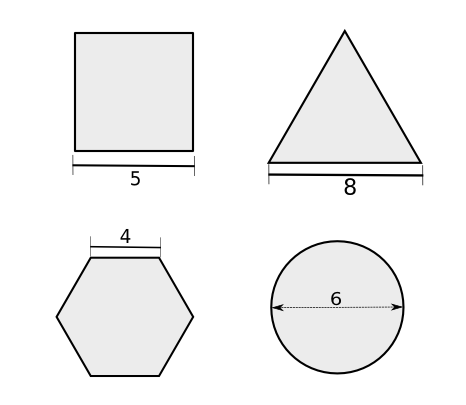
\includegraphics[scale=0.5]{all.png}
\end{figure}
\vspace{2cm}\\
¿Cuánto mide la suma de los ángulos internos de un triángulo?
\vspace{1.5cm}\\
Encuantra $x$ Usando el teorema de Pitágoras
\begin{figure}[h!]
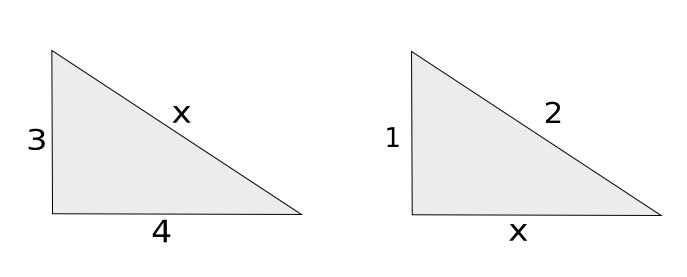
\includegraphics[scale=0.5]{pitagoras.png}
\end{figure}

\pagebreak

\subsection*{Funciones y geometría analítica}

Tabula los valores de la siguiente función  $y=\frac{3}{4}x+3$
\vspace{.5cm}\\
\begin{tabular}{|c|c|}\hline
$x$ & $y$ \\ \hline
 -2   &      \\ \hline
 -1   &      \\ \hline
 0   &       \\ \hline
 1   &       \\ \hline
4   &       \\ \hline
\end{tabular}
\vspace{0.5cm}\\

Grafica la función anterior y la función $y=-2x+7$
\begin{figure}[H]
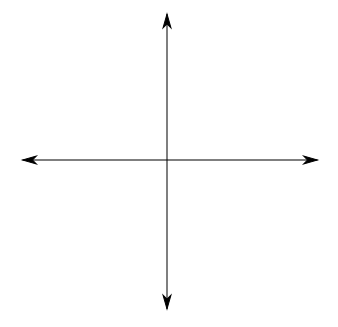
\includegraphics[scale=0.5]{plot.png}
\end{figure}
\vspace{0.5cm}\\

Encuentra la solución al siguiente sistema de ecuaciones y grafica:
\left\{\begin{tabular}{l}
$y=2x+5$\\
$y=-\frac{1}{3}x+4$\\
\end{tabular}\right\.

\begin{figure}[H]
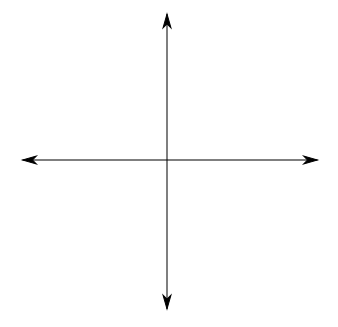
\includegraphics[scale=0.5]{plot.png}
\end{figure}
\vspace{0.5cm}\\
\pagebreak
Tabula los valores de la siguiente función  $y=\frac3x^2+2$
\vspace{.5cm}\\
\begin{tabular}{|c|c|}\hline
$x$ & $y$ \\ \hline
 -4   &      \\ \hline
 -2   &      \\ \hline
 0   &       \\ \hline
 1   &       \\ \hline
4   &       \\ \hline
\end{tabular}
\vspace{0.5cm}\\

Resuelve y grafica el siguiente sistema de ecuaciones:
\left\{\begin{tabular}{l}
$y=2x+5$\\
$y=-x^2+4$\\
\end{tabular}\right\.

\begin{figure}[H]
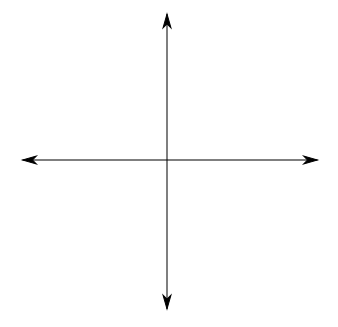
\includegraphics[scale=0.5]{plot.png}
\end{figure}
\vspace{0.5cm}\\

Identifica el lugar geométrico que representan las siguientes funciones y grafica:
\vspace{0.4cm}\\
$x^2+y^2=9$\hspace{3cm}$\frac{x^2}{4}+\frac{y^2}{16}=1$\hspace{3cm} $y-x^2=4$

\begin{figure}[H]
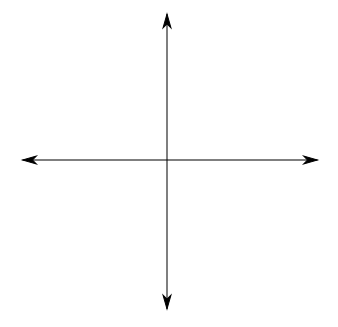
\includegraphics[scale=0.33]{plot.png}
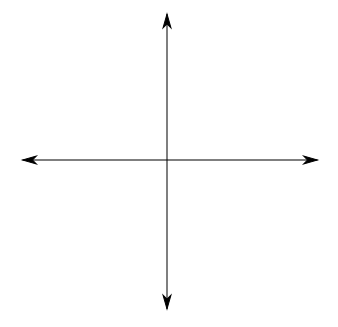
\includegraphics[scale=0.33]{plot.png}
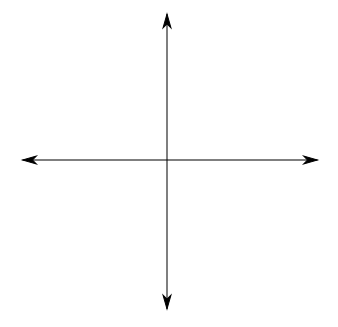
\includegraphics[scale=0.33]{plot.png}
\end{figure}
\vspace{0.5cm}\\

\pagebreak
Grafica las siguiente funciones.\\
$y=x^3$\hspace{1.3cm} $y=e^x$\hspace{1.3cm} $y=\log(x)$\hspace{1.3cm} $y=\sqrt{x}$\hspace{1.3cm} $y=\sin{x}$

\begin{figure}[H]
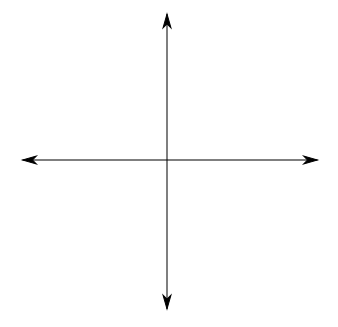
\includegraphics[scale=0.5]{plot.png}
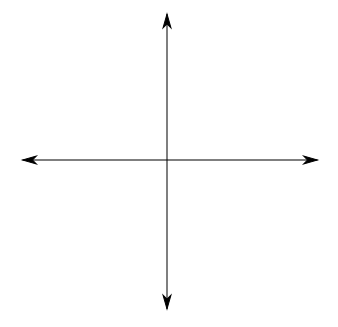
\includegraphics[scale=0.5]{plot.png}
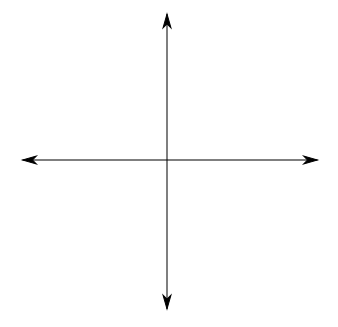
\includegraphics[scale=0.5]{plot.png}
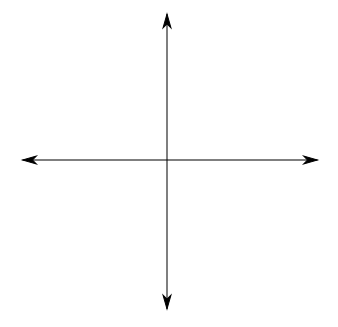
\includegraphics[scale=0.5]{plot.png}
\end{figure}
\vspace{0.5cm}\\
\subsection*{Cálculo diferencial}
Expreza con tus propias palabras el concepto de derivada.
\vspace{3cm}\\
Deriva las siguientes funciones con respecto a $x$:
\vspace{0.5cm}\\
$x^3+5x^2+x+10=$\hspace{3cm}$(3x+2)(x^2+5)=$\hspace{3cm}
\vspace{1cm}\\
$(3x^2+4)^3=$\hspace{4cm}$\frac{3x^2+4}{x+2}=$
\vspace{1.5cm}\\
$2\cos(5x)=$\hspace{4cm}$3e^x=$
\vspace{1.5cm}\\
$sin^3(5x^2)$\hspace{4cm}$3e^{7x^2+1}=$
\vspace{1.5cm}\\
Encuentra la recta tangente a $y=2\sin(x)$ en el punto $(0,0)$ y grafica.
\begin{figure}[H]
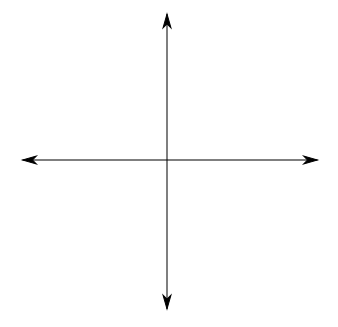
\includegraphics[scale=0.5]{plot.png}
\end{figure}
\pagebreak
Encuentra las raíces, y los máximos y mínimos locales de $y=x^3+12x+3$, grafica la función y señala los puntos encontrados. 
\begin{figure}[H]
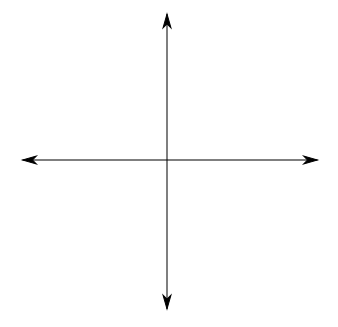
\includegraphics[scale=0.6]{plot.png}
\end{figure}
\pagebreak
\subsection*{Cálculo integral}
Expreza con tus propias palabras el concepto de integral. 
\vspace{3cm}\\
Integra las siguientes funciones:
\vspace{0.5cm}\\
$\int x^2+3x+5\; dx=$\hspace{4cm} $\int\sin(x)dx=$
\vspace{1.5cm}\\
$\int e^x dx=$ \hspace{4cm}}$\int \log (x) dx=$
\vspace{1.5cm}\\
$\int_2^3 3x^2+2x \; dx$
\vspace{2.5cm}$$\\
$\int e^x(3x^2+2x+1)dx$


\end{document}

